%%----------------------------------------------------------------------
%%----------------------------------------------------------------------
\missiontitle{Mission 2: Hardpoint}

%\teaser{Recon forces desperately searching for weaknesses in the enemy
%  lines collide!}

This is an asymmetric mission; players alternate games as the
\textbf{Attacker} and the \textbf{Defender}.

%%----------------------------------------------
  \begin{columns}
\begin{tablesetup}    
  There is no roll-off for deployment zones.  The Defender begins by
  choosing their player table edge and a corner of the board.  Their
  deployment zone is the 18''x18'' box in that corner.  The Attacker's
  player table edge is that opposite the Defender's.  Their deployment
  zone is 6'' along both table edges not incident to the Defender's
  corner.

  Place a primary objective marker 9'' by 9'' from each table corner,
  and a fifth at table center.  Label the marker in the Defender's
  deployment zone \#1, at table center \#2, and the others \#s 3--5 in
  any order.

  Roll off for deployment order and determine turn order as usual
  (first to deploy chooses turn order).
\end{tablesetup}

\vspace{1.5em}
\missionheading{Mission Specific Rules}
\vspace{-0.5em}
\nightfighting

\vfill\vbox to 0pt{}
\columnbreak
\bigskip\centerline{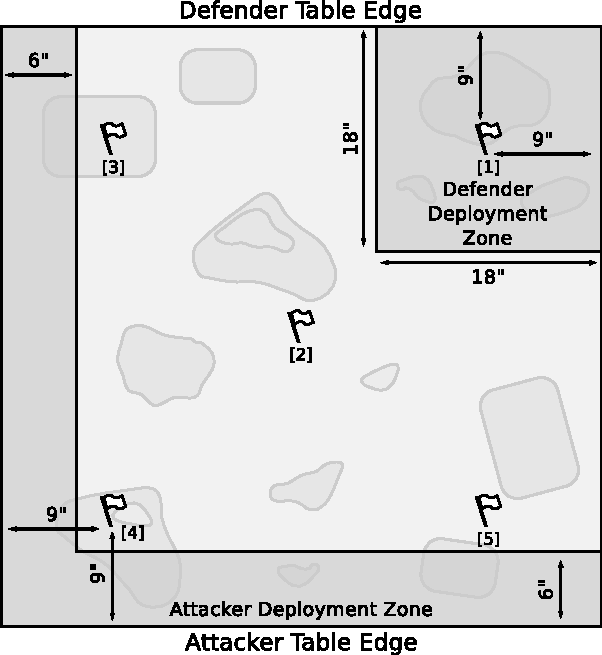
\includegraphics[width=\linewidth]{maps/mission2.pdf}}
  \end{columns}

\vspace{-2.5em}

\missionsubheading{Security Patrol.} During deployment the Defender
may grant the Infiltrate special rule to up to~3 of their units
(embarked units do not count).  These units do not gain Outflank and
may not be deployed in reserve.

\missionsubheading{Surrounded.} Attacker units arriving from reserve
may move onto the board from either full table edge along their
deployment zone (i.e., not the 6'' extents).  The table edge does not
have to be declared in advance.

%%----------------------------------------------
%\begin{missionrules}

%\end{missionrules}


%%----------------------------------------------
\begin{scoring}
  
\begin{primaries}

  Simultaneously with declaring secondary objectives, both players
  choose and declare three of the following primary scoring mechanisms
  for themselves, \underline{earning at most 9 victory points}:

  \begin{enumerate}[label=\Alph*.]\shortlist
  \item Control primary objective marker~\#1 at game end for~3 victory
    points.
  \item Control primary objective marker~\#2 at game end for~3 victory
    points.
  \item Earn~1 victory point at game end for each primary objective
    marker controlled of~\#s~3,~4, and~5.

  \item Earn~3 victory points if at least 25\% of the opposing army by
    units is broken.

  \item Earn~3 victory points if at least 50\% of the opposing army by
    units is broken.

  \item Earn~1 victory point per quartile if at least 25\%, 50\%, and
    75\% of your army is \emph{not} broken.
  \end{enumerate}

  Units are considered broken if at game end they have been
  eliminated, are falling back, are in reserve, or have at most~25\%
  of their starting models remaining.

\end{primaries}

\end{scoring}
